\documentclass[hyperref={pdfpagelabels=false}]{beamer}

\usepackage{xeCJK}
\setCJKmainfont[AutoFakeSlant=0.25]{Noto Sans Mono CJK SC}
\setCJKsansfont[AutoFakeSlant=0.25]{Noto Sans Mono CJK SC}
\setCJKmonofont[AutoFakeSlant=0.25]{Noto Sans Mono CJK SC}

\setbeamertemplate{bibliography item}[text]

\usepackage{lmodern}
\usepackage{datetime}
\usetheme{Madrid}
\usecolortheme{dolphin}
\title{基于强化学习的路由算法}  
\author{叶茂青} 

\date{\today}

\begin{document}
\begin{frame}
\titlepage
\end{frame} 

\begin{frame}
	\frametitle{总览}
	\tableofcontents
\end{frame} 

\section{问题描述}

\begin{frame}
	\frametitle{路由算法}
	路由算法用于引导网络流量,选定起始点和目的地,路由算法可以给出一组路径,指导路由器对流量进行转发,从而高效的利用网络资源。传统的路由算法有Link-state算法、Distance vector算法等。但传统的路由算法在收敛速度,可扩展性,算法复杂度等方面或多或少存在缺陷,利用机器学习的方法设计路由算法,或许能改善当前算法的缺陷,提高网络资源的利用率。
\end{frame}


\section{模型描述}

\begin{frame}
	\frametitle{模型描述}
	以下模型参考Boyan et al.\cite{boyan1994packet}提出的基于Q-Learning的路由算法进行建模,并对模型作出了下列改进:
	\begin{itemize}
		\item 考虑到掉包的可能,修改状态转移矩阵
		\item 对回报函数进行修改,避免模型一直选择最短路径
		\item 考虑到在线学习的可能性,加入监测机制,避免模型造成灾难性的后果
	\end{itemize}

\end{frame}

\subsection{优化目标}
\begin{frame}
	\frametitle{优化目标}
	路由算法的目的在于找出两点之间的最短路径,也就是使传输时间最小,设$Q_x(d,y)$表示从节点$x$到节点$d$的过程中,通过节点$y$所用的时间,当数据包传送到节点$y$时,节点$y$返回到达下一个节点预估时间给节点$x$,记为$t$,则
	\[
		t=\min _{z \in \text { neighbors of } y} Q_{y}(d, z)
	\]
	可定义Q表更新的值为,其中$q$为在节点$x$的排队时间,$s$为传输所用的时间,$\eta$为学习率
	\[
		\Delta Q_{x}(d, y)=\eta(\overbrace{q+s+t}^{\text {new estimate }}-\overbrace{Q_{x}(d, y)}^{\text {old estimate }})
	\]
\end{frame}

\subsection{状态及动作空间}
\begin{frame}
	\frametitle{状态及动作空间}
	路由算法的状态空间为所有路由器的集合,动作空间为路由器选择转发到哪个路由器,考虑到网络中可能存在掉包的可能,设$P_{s_1,s_2}$为从路由器1到达路由器2成功的概率,则应掉包等原因传输失败的概率为$1-P_{s_1,s_2}$,则下图的网络结构的状态转移矩阵P可表示为

	\begin{table}[]\small
		\begin{tabular}{|l|l|l|l|}
		\hline
		      & $s_1$                             & $s_2$                              & $s_3$ \\ \hline
		$s_1$ & $1-P_{s_1,s_2}\ or\ 1 -P_{s_1,s_3}$  & $P_{s_2,s_1}$                      & $P_{s_3,s_1}$  \\ \hline
		$s_2$ & $P_{s_1,s_2}$                     & $1-P_{s_2,s_1}\ or\ 1-P_{s_2,s_3}$   & $P_{s_3,s_2}$  \\ \hline
		$s_3$ & $P_{s_1,s_3}$                     & $P_{s_2,s_3}$                      & $1-P_{s_3,s_1}\ or\ 1-P_{s_3,s_2}$  \\ \hline
		\end{tabular}
	\end{table}

	\begin{figure}
		\centering
		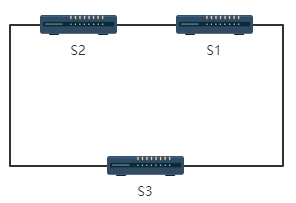
\includegraphics[width=.4\textwidth]{./figure/1.png}
	\end{figure}
\end{frame}



\subsection{回报函数}
\begin{frame}
	\frametitle{回报函数}
	根据之前的描述,Boyan et al.\cite{boyan1994packet}提出的模型的回报函数可看作为$-(q+s+t)$,其中的$t$相当于奖励模型寻找最短路径,而$q+s$使得模型可以感知到拥塞的发生,并让模型对Q表进行调整,当网络结构较为庞大时,要让模型更新Q表以重新收敛需要很长的时间,这会使得模型在某些情况下变得不稳定。针对这一点,可以在回报函数中显式的添加对网络拥塞程度的估计,即在回报函数中添加$\alpha l$这一项,其中$\alpha$用于控制惩罚的程度,$l$为当前节点带宽的使用率,使得节点偏向于选择负载低的节点,此时的回报函数为$-(q+s+t+\alpha l)$,Q表更新的值变为
	\[
		\Delta Q_{x}(d, y)=\eta(q+s+t+\alpha l-Q_{x}(d, y))
	\]
\end{frame}

\subsection{监测系统}
\begin{frame}
	\frametitle{监测系统}
	Boyan et al.\cite{boyan1994packet}提出的模型使用离线学习的方法,这样做可以避免模型在学习过程中随意探索导致的灾难性行为,比如引发回路,或将数据包发送到不应该发送的地方,但虚拟的环境与实际的环境可能并不一致,且想要对实际环境进行精确的建模也较为困难,如果能将模型放到实际的环境中便能解决这个问题。为了避免模型在探索过程对网络造成破坏,我们可以引入监测系统评判模型的行为是否会导致回路等问题,如果存在安全风险,则应该让模型回到上一个状态,并对该决策做出惩罚,从而保证网络的安全。
\end{frame}




\begin{frame}[allowframebreaks]
	\frametitle{References}
	\bibliographystyle{IEEEtran}
	\bibliography{ppt.bib}
\end{frame}

\end{document}

